% !TeX spellcheck = en_GB
\chapter{The Haagerup subfactor and its fusion categories}
\label{ch:Haagerup}

In the study of exotic subfactors, it is natural to ask what the subfactor with the smallest possible index above four is. In \cite{Haagerup1994}, Haagerup investigated this problem by analysing the principal graphs of subfactors with small indices above four. More precisely, he asked the question which non-trivial principal graphs with index near four (in fact, with index in the range $(4,3+\sqrt{3})$) are possible, i.e., have a subfactor associated to them. As a result, he found that there cannot be a subfactor with index in the interval $(4,\frac{5+\sqrt{13}}{2})$, and provides a list with possible pairs of principal graphs\footnote{Note that the pair $(\Gamma,\Gamma')$ of principal graphs is unordered since any subfactor $N\subseteq M$ has a dual with the same index but where the principal and dual principal graph are switched.} in the range $[\frac{5+\sqrt{13}}{2},3+\sqrt{3})$:
{{\setlength{\tabcolsep}{7pt}
		\renewcommand{\arraystretch}{2.5}
		\begin{table}[H]
			\centering
			\begin{tabular}{c|c|c}
				& principal graph $\Gamma$& Dual principal graph $\Gamma'$\\\hline
				$\mathcal{H}_n$ & 
				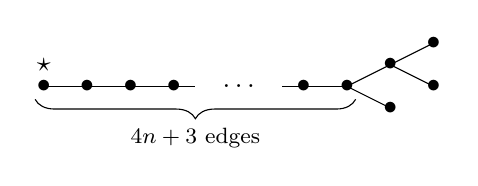
\begin{tikzpicture}[baseline=(current bounding box.center),scale=1.1]
				\draw (0,0) -- (1.75,0);
				\node at (2.25,0) {$\dots$};
				\draw (2.75,0) -- (3.5,0);
				\draw (3.5,0) -- (4.5,0.5);
				\draw (4,0.25) -- (4.5,0);
				\draw (3.5,0) -- (4,-0.25);
				\foreach \a in {0,0.5,1,1.5,3,3.5}{
					\node at (\a,0) {$\bullet$};
				}
				\node at (4,0.25) {$\bullet$};
				\node at (4.5,0.5) {$\bullet$};
				\node at (4.5,0) {$\bullet$};
				\node at (4,-0.25) {$\bullet$};
				\draw[decorate,decoration={brace,amplitude=7pt}] (3.6,-0.15) -- (-0.1,-0.15);
				\node at (1.75,-0.6) {\footnotesize $4n+3$ edges};
				\node at (0,0.25) {$\star$};
				\end{tikzpicture}& 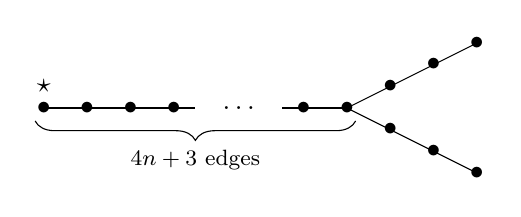
\begin{tikzpicture}[baseline=(current bounding box.center),scale=1.1]
				\draw (0,0) -- (1.75,0);
				\node at (2.25,0) {$\dots$};
				\draw (2.75,0) -- (3.5,0);
				\draw (3.5,0) -- (5,0.75);
				\draw (3.5,0) -- (5,-0.75);
				\foreach \a in {0,0.5,1,1.5,3,3.5}{
					\node at (\a,0) {$\bullet$};
				}
				\node at (4,0.25) {$\bullet$};
				\node at (4.5,0.5) {$\bullet$};
				\node at (5,0.75) {$\bullet$};
				\node at (4,-0.25) {$\bullet$};
				\node at (4.5,-0.5) {$\bullet$};
				\node at (5,-0.75) {$\bullet$};
				\draw[decorate,decoration={brace,amplitude=7pt}] (3.6,-0.15) -- (-0.1,-0.15);
				\node at (1.75,-0.6) {\footnotesize $4n+3$ edges};
				\node at (0,0.25) {$\star$};
				\end{tikzpicture}
				\\
				$\mathcal{B}_n$ & 
				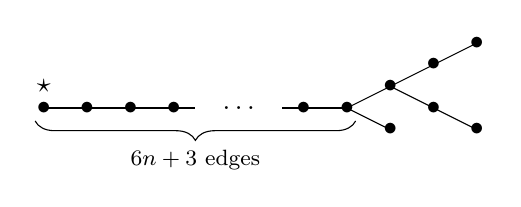
\begin{tikzpicture}[baseline=(current bounding box.center),scale=1.1]
				\draw (0,0) -- (1.75,0);
				\node at (2.25,0) {$\dots$};
				\draw (2.75,0) -- (3.5,0);
				\draw (3.5,0) -- (5,0.75);
				\draw (4,0.25) -- (5,-0.25);
				\draw (3.5,0) -- (4,-0.25);
				\foreach \a in {0,0.5,1,1.5,3,3.5}{
					\node at (\a,0) {$\bullet$};
				}
				\node at (4,0.25) {$\bullet$};
				\node at (4.5,0.5) {$\bullet$};
				\node at (4.5,0) {$\bullet$};
				\node at (4,-0.25) {$\bullet$};
				\node at (5,0.75) {$\bullet$};
				\node at (5,-0.25) {$\bullet$};
				\draw[decorate,decoration={brace,amplitude=7pt}] (3.6,-0.15) -- (-0.1,-0.15);
				\node at (1.75,-0.6) {\footnotesize $6n+3$ edges};
				\node at (0,0.25) {$\star$};
				\end{tikzpicture} & 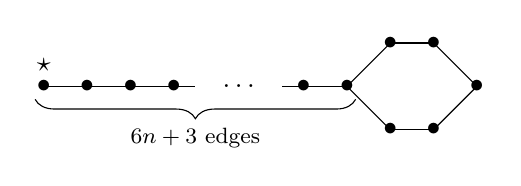
\begin{tikzpicture}[baseline=(current bounding box.center),scale=1.1]
				\draw (0,0) -- (1.75,0);
				\node at (2.25,0) {$\dots$};
				\draw (2.75,0) -- (3.5,0);
				\draw (3.5,0) -- (4,0.5);
				\draw (4,0.5) -- (4.5,0.5);
				\draw (4.5,0.5) -- (5,0);
				\draw (3.5,0) -- (4,-0.5);
				\draw (4,-0.5) -- (4.5,-0.5);
				\draw (4.5,-0.5) -- (5,0);
				\foreach \a in {0,0.5,1,1.5,3,3.5}{
					\node at (\a,0) {$\bullet$};
				}
				\node at (4,0.5) {$\bullet$};
				\node at (4.5,0.5) {$\bullet$};
				\node at (4.5,-0.5) {$\bullet$};
				\node at (4,-0.5) {$\bullet$};
				\node at (5,0) {$\bullet$};
				\draw[decorate,decoration={brace,amplitude=7pt}] (3.6,-0.15) -- (-0.1,-0.15);
				\node at (1.75,-0.6) {\footnotesize $6n+3$ edges};
				\node at (0,0.25) {$\star$};
				\end{tikzpicture}\\
				$\mathcal{AH}$  &
				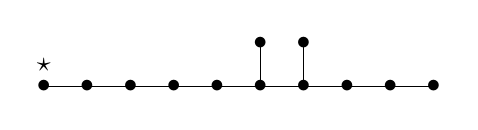
\begin{tikzpicture}[baseline=(current bounding box.center),scale=1.1]
				\draw (0,0) -- (4.5,0);
				\foreach \a in {0,0.5,...,4.5}{
					\node at (\a,0) {$\bullet$};
				}
				\node at (0,0.25) {$\star$};
				\draw (2.5,0) -- (2.5,0.5);
				\draw (3,0) -- (3,0.5);
				\node at (2.5,0.5) {$\bullet$};
				\node at (3,0.5) {$\bullet$};
				\end{tikzpicture} & 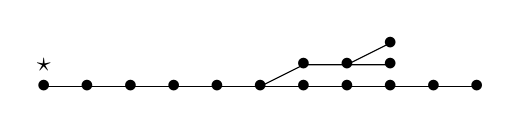
\begin{tikzpicture}[baseline=(current bounding box.center),scale=1.1]
				\draw (0,0) -- (5,0);
				\foreach \a in {0,0.5,...,5}{
					\node at (\a,0) {$\bullet$};
				}
				\node at (0,0.25) {$\star$};
				\draw (2.5,0) -- (3,0.25) -- (4,0.25);
				\draw (3.5,0.25) -- (4,0.5);
				\node at (3,0.25) {$\bullet$};
				\node at (3.5,0.25) {$\bullet$};
				\node at (4,0.25) {$\bullet$};
				\node at (4,0.5) {$\bullet$};
				\end{tikzpicture}
			\end{tabular}
	\end{table}}
	\vspace{8pt}
	Here, $\mathcal{H}_n$ and $\mathcal{B}_n$ are infinite families of potential subfactors, where $n\in\mathbb{N}$. The indices of the subfactors that correspond to these graphs range from $\mathrm{index}(\mathcal{H}_0)=\frac{5+\sqrt{13}}{2}\approx4.30278$ to $\lim_{n\to\infty}\mathrm{index}(\mathcal{B}_n)\approx 4.65897$. 
	
	However, even though these principal graphs are \emph{possible} graphs, it does not automatically mean that they are realized by a subfactor. While Haagerup's original result did not specify which graphs are actually realized, this question was investigated by various scientists in the subsequent years. It was shown by Haagerup and Asaeda \cite{asaeda_exotic_1999} that the graph $\mathcal{H}_0$ (the \emph{Haagerup subfactor}\index{Haagerup subfactor}) as well as the graph $\mathcal{AH}$ (the \emph{Asaeda-Haagerup subfactor})\index{Asaeda-Haagerup subfactor} are realized by subfactors. An alternative construction of the Haagerup subfactor via a system of endomorphisms of a certain Cuntz algebra by Izumi is given in \cite{izumi_structure_2001}. Additionally, a construction of the Haagerup subfactor via so-called \emph{planar algebras} was presented by Peters in \cite{Peters2010}. Furthermore, it was shown by Bisch \cite{Bisch1998} that none of the graphs $\mathcal{B}_n$ can be the principal graphs of a subfactor since they yield inconsistent fusion rules, and Asaeda and Yasuda \cite{Asaeda2007,Asaeda2008} proved that $\mathcal{H}_n$ is not the principal graph of a subfactor for $n\ge 2$, which only left the existence of a subfactor with principal graph $\mathcal{H}_1$ as an open problem. The classification of subfactors up to index $3+\sqrt{3}$ was completed when it was shown in \cite{bigelow_constructing_2012} that $\mathcal{H}_1$ is realized by the so-called \emph{extended Haagerup subfactor}\index{extended Haagerup subfactor}, using a construction via subfactor planar algebras.
	
	In this thesis, we focus on the subfactor that corresponds to $\mathcal{H}_0$, which is the Haagerup subfactor, and the fusion categories that can be constructed from it. For this purpose, let us analyse the principal and dual principal graph in terms of their respective even and odd parts. We begin with the principal graph $\Gamma$. Remember that $\Gamma_\mathrm{even}$ (respectively, $\Gamma_\mathrm{odd}$) is the set of vertices with even (respectively, odd) distance to the object $\star$. To emphasize this, the elements of $\Gamma_\mathrm{even}$ are coloured red and the elements of $\Gamma_\mathrm{odd}$ are coloured blue in the following figure:
	\begin{figure}[H]
		\centering
		\begin{tikzpicture}[baseline=(current bounding box.center),scale=2.5]
			\draw (2,0) -- (3.5,0);
			\draw (3.5,0) -- (4.5,0.5);
			\draw (4,0.25) -- (4.5,0);
			\draw (3.5,0) -- (4,-0.25);
			\foreach \a in {2,3}{
				\node at (\a,0) {\color{LinkColor}\Large$\bullet$};
			}
			\node at (2.5,0) {\color{LinkColor2}\Large$\bullet$};
			\node at (3.5,0) {\color{LinkColor2}\Large$\bullet$};
			\node at (4,0.25) {\color{LinkColor}\Large$\bullet$};
			\node at (4.5,0.5) {\color{LinkColor2}\Large$\bullet$};
			\node at (4.5,0) {\color{LinkColor2}\Large$\bullet$};
			\node at (4,-0.25) {\color{LinkColor}\Large$\bullet$};
			\node at (2,-0.15) {$\mathbf{1}$};
			%			\node at (2.5,-0.15) {$\kappa$};
			\node at (3,-0.15) {$\eta$};
			%			\node at (3.5,-0.2) {$\lambda$};
			\node at (4,-0.4) {$\mu$};
			\node at (4,0.4) {$\nu$};
			%			\draw[decorate,decoration={brace,amplitude=7pt}] (3.6,-0.15) -- (-0.1,-0.15);
			%			\node at (1.75,-0.6) {\footnotesize $4n+3$ edges};
			%			\node at (0,0.25) {$\star$};
		\end{tikzpicture}
	\end{figure}
	The elements of $\Gamma_\mathrm{even}$ are equipped with labels that denote the object in the corresponding fusion category, which we denote $\mathcal{H}_1$\footnote{Be aware that this notation has nothing to do with the $\mathcal{H}_n$ that denoted the possible principal graphs in Haagerup's list. From now on, we use $\mathcal{H}_i$ with $i\in\{1,2,3\}$ to denote the three different categories in the Morita equivalence class of categories associated to the Haagerup subfactor.}. According to the fusion graph, this category has four simple objects: $\Obj(\mathcal{H}_1)=\{\mathbf{1},\eta,\nu,\mu\}$ with quantum dimensions 
	\begin{equation}
	\dim(\mathbf{1})=1,\hspace{10pt}\dim(\eta)=\frac{3+\sqrt{13}}{2},\hspace{10pt}\dim(\nu)=\frac{1+\sqrt{13}}{2},\hspace{10pt}\dim(\mu)=\frac{5+\sqrt{13}}{2}.
	\end{equation}
	The corresponding fusion rules $X\otimes Y=\sum_Z N_{XY}^Z Z$ for $X,Y,Z\in\Obj(\mathcal{H}_1)$ are listed in \cref{tab:fusionH1}:
	{{\setlength{\tabcolsep}{10pt}
		\renewcommand{\arraystretch}{1.25}
		\begin{table}[H]
			\centering
			\begin{tabular}{c||c|c|c|c}
				& $\mathbf{1}$ & $\nu$ & $\eta$ & $\mu$  \\ \hline \hline
				$\mathbf{1}$ & $\mathbf{1}$ & $\nu$ & $\eta$ & $\mu$\\ \hline
				$\nu$ & $\nu$ & $\mathbf{1}+2\nu+2\eta+\mu$ & $2\nu+\eta+\mu$ & $\nu+\eta+\mu$  \\ \hline
				$\eta$ & $\eta$ & $2\nu+\eta+\mu$ & $\mathbf{1}+\nu+\eta+\mu$ & $\nu+\eta$  \\ \hline
				$\mu$ & $\mu$ & $\nu+\eta+\mu$ & $\nu+\eta$ & $\mathbf{1}+\nu$\vspace{8pt}
			\end{tabular}
			\caption{\small \label{tab:fusionH1}Fusion rules for the $\mathcal{H}_1$ fusion category.}
		\end{table}}
		
		In the same fashion we can analyse the dual principal graph $\Gamma'$ whose even part $\Gamma_\mathrm{even}'$ gives rise to the fusion category $\mathcal{H}_2$. As above, even vertices are coloured red and odd vertices are coloured blue, and we add labels to those vertices that correspond to objects in the fusion category.
		\begin{figure}[H]
			\centering
			\begin{tikzpicture}[baseline=(current bounding box.center),scale=2.5]
			\draw (2,0) -- (3.5,0);
			\draw (3.5,0) -- (5,0.75);
			\draw (3.5,0) -- (5,-0.75);
			\node at (2,0) {\color{LinkColor}\Large$\bullet$};
			\node at (2.5,0) {\color{LinkColor2}\Large$\bullet$};
			\node at (3,0) {\color{LinkColor}\Large$\bullet$};
			\node at (3.5,0) {\color{LinkColor2}\Large$\bullet$};
			\node at (4,0.25) {\color{LinkColor}\Large$\bullet$};
			\node at (4.5,0.5) {\color{LinkColor2}\Large$\bullet$};
			\node at (5,0.75) {\color{LinkColor}\Large$\bullet$};
			\node at (4,-0.25) {\color{LinkColor}\Large$\bullet$};
			\node at (4.5,-0.5) {\color{LinkColor2}\Large$\bullet$};
			\node at (5,-0.75) {\color{LinkColor}\Large$\bullet$};
			\node at (2,-0.15) {$\mathbf{1}$};
			\node at (3,-0.15) {$\rho$};
			\node at (4,-0.4) {${}_\alpha\rho$}; 
			\node at (5,-0.9) {$\alpha$}; 
			\node at (4,0.4) {$\alphastarrho$}; 
			\node at (5,0.9) {$\alpha^*$}; 
			\end{tikzpicture}
		\end{figure}
		
		Hence, the fusion category $\mathcal{H}_2$ has six simple objects: $\Obj(\mathcal{H}_2)=\{\mathbf{1},\alpha,\alpha^*,\rho,{}_\alpha\rho,\alphastarrho\}$ with the following quantum dimensions:
		\begin{align}
		\dim(\mathbf{1})=\dim(\alpha)=\dim(\alpha^*)=1,\hspace{10pt}\dim(\rho)=\dim({}_\alpha\rho)=\dim(\alphastarrho)=\frac{3+\sqrt{13}}{2}.
		\end{align}
		and fusion rules given in \cref{tab:fusionH2}:
		{{\setlength{\tabcolsep}{10pt}
			\renewcommand{\arraystretch}{1.25}
			\begin{table}[H]
				\centering
				\begin{tabular}{c||c|c|c|c|c|c}
					& $\mathbf{1}$ & $\alpha$ & $\alpha^*$ & $\rho$ & ${}_\alpha
					\rho$ & $\alphastarrho$ \\ \hline \hline
					$\mathbf{1}$ & $\mathbf{1}$ & $\alpha$ & $\alpha^*$ & $\rho$ & ${}_\alpha \rho$ & $\alphastarrho$ \\ \hline
					$\alpha$ & $\alpha$ & $\alpha^*$ & $\mathbf{1}$ & ${}_\alpha \rho$ & $\alphastarrho$ & $\rho$ \\ \hline
					$\alpha^*$ & $\alpha^*$ & $\mathbf{1}$ & $\alpha$ & $\alphastarrho$ & $\rho$ & ${}_\alpha \rho$ \\ \hline
					$\rho$ & $\rho$ & $\alphastarrho$ & ${}_\alpha \rho$ & $\mathbf{1}+ Z$ & $\alpha^*+Z$ & $\alpha+Z$ \\ \hline
					${}_\alpha\rho$ & ${}_\alpha\rho$ & $\rho$ & $\alphastarrho$ & $\alpha+Z$ & $\mathbf{1}+Z$ & $\alpha^*+Z$ \\ \hline
					$\alphastarrho$ & $\alphastarrho$ & ${}_\alpha\rho$ & $\rho$ & $\alpha^*+Z$ & $\alpha+Z$ & $\mathbf{1}+Z$\vspace{8pt}
				\end{tabular}
				\caption{\small \label{tab:fusionH2}Fusion rules for the $\mathcal{H}_2$ and $\mathcal{H}_3$ fusion category, with $Z=\rho+{}_\alpha\rho+\alphastarrho$.}
			\end{table}}
			
			Since these two categories arise as the principal even and the dual even part of the same subfactor, they are Morita equivalent. This implies that there is an algebra object $A_1\in\mathcal{H}_1$ such that $\mathcal{H}_2$ is isomorphic to the category of $A_1$--$A_1$ bimodules over $\mathcal{H}_1$. On the other hand, there is an algebra object $A_2\in\mathcal{H}_2$ such that $\mathcal{H}_1$ is isomorphic to the category of $A_2$--$A_2$ bimodules over $\mathcal{H}_2$. In \cite{grossman_quantum_2012}, this connection was studied in detail and found that the algebra object $A_1\in\mathcal{H}_1$ is $\mathbf{1}+\eta$, and the algebra object $A_2\in\mathcal{H}_2$ is $\mathbf{1}+\rho$.
			
			Moreover, the authors of \cite{grossman_quantum_2012} exploited this technique to determine all fusion categories in the Morita equivalence class of $\mathcal{H}_1$ and $\mathcal{H}_2$ and found that there is exactly one additional category in this class, denoted $\mathcal{H}_3$. It has the same simple objects and fusion rules as $\mathcal{H}_2$ (see \cref{tab:fusionH2}). It can be constructed as the category of $(\mathbf{1}+\alpha+\alpha^*)-(\mathbf{1}+\alpha+\alpha^*)$ bimodules over $\mathcal{H}_2$ or as the category of $(\mathbf{1}+\mu+\nu)-(\mathbf{1}+\mu+\nu)$ bimodules over $\mathcal{H}_1$. The Morita equivalence class is summarized in \cref{fig:MoritaH}.
			\begin{figure}[H]
				\centering
				\begin{tikzpicture}[scale=3]
				\node (H1) at (0,0) {\color{LinkColor2}\huge$\mathcal{H}_1$};
				\node (H2) at (3,0) {\color{LinkColor3}\huge$\mathcal{H}_2$};
				\node (H3) at (1.5,-1.5) {\color{LinkColor}\huge$\mathcal{H}_3$};
				\draw[->,>=stealth,thick,color=LinkColor2] (0.3,0.05) to node[above] {\large$\mathbf{1}+\eta$} (2.7,0.05);
				\draw[->,>=stealth,thick,color=LinkColor3] (2.7,-0.05) to node[below] {\large$\mathbf{1}+\rho$} (0.3,-0.05);
				\draw[->,>=stealth,thick,color=LinkColor] (1.6,-1.3) to node[left,pos=0.6] {\large$\mathbf{1}+\alpha+\alpha^*\ $} (2.8,-0.2);
				\draw[->,>=stealth,thick,color=LinkColor3] (2.95,-0.2) to node[right,pos=0.6] {\large$\ \mathbf{1}+\alpha+\alpha^*$} (1.7,-1.35);
				\draw[->,>=stealth,thick,color=LinkColor2] (0.2,-0.2) to node[right,pos=0.4] {\large$\ \mathbf{1}+\mu+\nu$} (1.4,-1.3);
				\draw[->,>=stealth,thick,color=LinkColor] (1.3,-1.35) to node[left,pos=0.4] {\large$\mathbf{1}+\rho+{}_\alpha\rho\ $} (0.05,-0.2);
				\end{tikzpicture}
				\caption{\small \label{fig:MoritaH}The Morita equivalence class of fusion categories coming from the Haagerup subfactor. The object on the arrow from $\mathcal{H}_i$ to $\mathcal{H}_j$ indicates the algebra object $A$ from which $\mathcal{H}_j$ can be built as the category of $A$-$A$ bimodules over $\mathcal{H}_i$.}
			\end{figure}
			
	\begin{exmp}
		Using the technique described in \cref{sec:AOtographs} we can recover the principal and dual graphs of the Haagerup subfactor from its fusion categories. The principal graph can be constructed via the module category $\mathsf{Mod}_{\mathcal{H}_1}(\mathbf{1}+\eta)$ and choosing $\mathbf{1}+\eta$ as the fixed simple module object therein. The dual graph can analogously be constructed via $\mathsf{Mod}_{\mathcal{H}_2}(\mathbf{1}+\rho)$ and choosing $\mathbf{1}+\rho$ as the fixed simple module object. We go through both constructions in detail, beginning with the principal graph. 
			
		To construct the principal graph of the Haagerup subfactor, we start with the algebra object $\mathbf{1}+\eta$ in $\Hi_1$. Recall that we first construct the matrix $T$ whose rows are determined by the decomposition of $ X_i\otimes(\mathbf{1}+\eta)$. The result is
			\begin{equation}
				T=\begin{blockarray}{ccccc}
				& \mathbf{1} & \nu & \eta & \mu \\
				\begin{block}{c (cccc)}
				\mathbf{1} & 1 & 0 & 1 & 0 \topstrut \\
				\nu & 0 & 3 & 1 & 1 \\
				\eta & 1 & 1 & 2 & 1 \\
				\mu & 0 & 1 & 1 & 1 \botstrut \\
				\end{block}
				\end{blockarray}\ .
			\end{equation}
		The matrix $V$ that fulfils $T=VV^\mathrm{T}$ is given by
			\begin{equation}
				V=\begin{pmatrix}
					1 & 0 & 0 & 0\\
					0 & 1 & 1 & 1\\
					1 & 1 & 0 & 0\\
					0 & 1 & 0 & 0
				\end{pmatrix}\ .
			\end{equation}
		Interpreting $V$ as an adjacency matrix yields the following graph
			\begin{equation}
				\begin{tikzpicture}[baseline=(current bounding box.center),scale=2]
				\draw (2,0) -- (3.5,0);
				\draw (3.5,0) -- (4.5,0.5);
				\draw (4,0.25) -- (4.5,0);
				\draw (3.5,0) -- (4,-0.25);
				\foreach \a in {2,3}{
					\node at (\a,0) {\color{LinkColor}\Large$\bullet$};
				}
				\node at (2.5,0) {\color{LinkColor2}\Large$\bullet$};
				\node at (3.5,0) {\color{LinkColor2}\Large$\bullet$};
				\node at (4,0.25) {\color{LinkColor}\Large$\bullet$};
				\node at (4.5,0.5) {\color{LinkColor2}\Large$\bullet$};
				\node at (4.5,0) {\color{LinkColor2}\Large$\bullet$};
				\node at (4,-0.25) {\color{LinkColor}\Large$\bullet$};
				\node at (2,-0.15) {\small $\mathbf{1}$};
				\node at (3,-0.15) {\small $\eta$};
				\node at (4,-0.4) {\small $\mu$};
				\node at (4,0.4) {\small $\nu$};
				\end{tikzpicture},
			\end{equation}
		which is exactly the principal graph of the Haagerup subfactor. For the calculation of the dual graph, we begin with the algebra object $\mathbf{1}+\rho$ in $\Hi_2$. The matrix $T$ constructed from the fusion outcomes of $X_i\otimes(\mathbf{1}+\rho)$ is given by
			\begin{equation}
				T=\begin{blockarray}{ccccccc}
				& \mathbf{1} & \alpha & \alpha^* & \rho & {}_\alpha\rho & \alphastarrho\\
				\begin{block}{c (cccccc)}
				\mathbf{1} & 1 & 0 & 0 & 1 & 0 & 0 \topstrut \\
				\alpha & 0 & 1 & 0 & 0 & 1 & 0\\
				\alpha^* & 0 & 0 & 1 & 0 & 0 & 1\\
				\rho & 1 & 0 & 0 & 2 & 1 & 1\\
				{}_\alpha\rho & 0 & 1 & 0 & 1 & 2 & 1\\
				\alphastarrho & 0 & 0 & 1 & 1 & 1 & 2\botstrut \\
				\end{block}
				\end{blockarray}\ ,
			\end{equation}
		and, therefore, $V$ is
			\begin{equation}
				V=\begin{pmatrix}
					1 & 0 & 0 & 0 \\
					0 & 1 & 0 & 0 \\
					0 & 0 & 1 & 0 \\
					1 & 0 & 0 & 1 \\
					0 & 1 & 0 & 1 \\
					0 & 0 & 1 & 1
				\end{pmatrix}.
			\end{equation}
		Note that, apart from interpreting $V$ directly as the adjacency matrix of the principal graph we can also read off the decomposition of the objects $M_i$ in the module category from this matrix:
			\begin{align}
				M_1&=\mathbf{1}+\rho\\
				M_2&=\alpha+\alpharho\\
				M_3&=\alpha^*+\alphastarrho\\
				M_4&=\rho+\alpharho+\alphastarrho.
			\end{align}
		The action $X_i\circlearrowright(\mathbf{1}+\rho)$ for $X_k\in\Obj(\mathcal{H}_2)$ is given by
			\begin{align}
				&\mathbf{1}\circlearrowright(\mathbf{1}+\rho)=\mathbf{1}+\rho=M_1\\
				&\alpha\circlearrowright(\mathbf{1}+\rho)=\alpha+\alpharho=M_2\\
				&\alpha^*\circlearrowright(\mathbf{1}+\rho)=\alpha^*+\alphastarrho=M_3\\
				&\rho\circlearrowright(\mathbf{1}+\rho)=\mathbf{1}+2\rho+\alpharho+\alphastarrho=M_1+M_4\\
				&\alpharho\circlearrowright(\mathbf{1}+\rho)=\alpha+\rho+2\alpharho+\alphastarrho=M_2+M_4\\
				&\alphastarrho\circlearrowright(\mathbf{1}+\rho)=\alpha^*+\rho+\alpharho+2\alphastarrho=M_3+M_4,
			\end{align} 
		which yields the following graph (where we can see that $V$ is indeed the adjacency matrix of this graph) which is the dual principal graph of the Haagerup subfactor:
%		with index $\dim(\mathbf{1}+\rho)=\frac{5+\sqrt{13}}{2}$,
			\begin{equation}
				\begin{tikzpicture}[baseline=(current bounding box.center),scale=2]
					\draw (2,0) -- (3.5,0);
					\draw (3.5,0) -- (5,0.75);
					\draw (3.5,0) -- (5,-0.75);
					\node at (2,0) {\color{LinkColor}\Large$\bullet$};
					\node at (2.5,0) {\color{LinkColor2}\Large$\bullet$};
					\node at (3,0) {\color{LinkColor}\Large$\bullet$};
					\node at (3.5,0) {\color{LinkColor2}\Large$\bullet$};
					\node at (4,0.25) {\color{LinkColor}\Large$\bullet$};
					\node at (4.5,0.5) {\color{LinkColor2}\Large$\bullet$};
					\node at (5,0.75) {\color{LinkColor}\Large$\bullet$};
					\node at (4,-0.25) {\color{LinkColor}\Large$\bullet$};
					\node at (4.5,-0.5) {\color{LinkColor2}\Large$\bullet$};
					\node at (5,-0.75) {\color{LinkColor}\Large$\bullet$};
					\node at (2,-0.15) {\small $\mathbf{1}$};
					\node at (3,-0.15) {\small $\rho$};
					\node at (4,-0.4) {\small $\alphastarrho$}; 
					\node at (5,-0.9) {\small $\alpha^*$}; 
					\node at (4,0.4) {\small $\alpharho$}; 
					\node at (5,0.9) {\small $\alpha$}; 
					\node at (2.5,-0.15) {\small $M_1$};
					\node at (3.5,-0.15) {\small $M_4$};
					\node at (4.5,0.65) {\small $M_2$};
					\node at (4.5,-0.65) {\small $M_3$};
				\end{tikzpicture}\ .
			\end{equation}
	\end{exmp}

\section{The $F$-symbols for the category $\Hd$}

	The $F$-symbols of a fusion category are important for any problem that involves working in a specific basis, for example the construction of module categories via algebra objects explained above. Moreover, they are a crucial ingredient in the construction of physical models from fusion categories such as one-dimensional spin chains or two-dimensional lattice models (presented in Part $2$ of this thesis). Especially for lattice models, we need the matrix representation of the $F$-symbols. Hence, even though the $F$-symbols are, in principal, obtained by Izumi's construction in \cite{izumi_structure_2001}, some work has to be done to obtain the corresponding matrix representation.
	
	A straightforward way to obtain the $F$-symbols of a given fusion category is to solve the pentagon equation \eqref{eq:pentagon}:
			\begin{equation}
			\label{eq:penta2}
				\left(F_u^{abr}\right)_{sp}\left(F_u^{pcd}\right)_{rq}=\sum_t \left(F_s^{bcd}\right)_{rt}\left(F_u^{atd}\right)_{sq}\left(F_q^{abc}\right)_{tp}.
			\end{equation}
	This equation has to be fulfiled for any combination of labels from the set of simple objects. Hence, the objective here is to solve a set of multivariate equations of polynomials up to third order, where the number of variables and equations is growing with the number of simple objects in the category. This task quickly becomes complicated if the number of simples in the category is too high, and explicit solutions are only known for a handful of cases (a list of many explicit solutions can, for example, be found in \cite{Bond2007}).
	
	In case of the fusion category $\mathcal{H}_3$ there are six simple objects, hence it presents no shortage of challenges: After eliminating trivial equations (i.e., those that contain non-valid $F$-symbols or those that are trivially true), there are $41391$ equations and $1431$ unknowns, resulting in a task that is at the limit of what is easily computable with current state-of-the-art technology and algorithms. To solve this problem, we use the following strategy: We first collect ``seed'' data about the $F$-symbols that can then be input to standard solvers in order to simplify the problem (the detailed description of the procedure can be found in \cite{Osborne2019}). This data comes from three different sources:
		\begin{enumerate}
			\item \textbf{Unitarity.} Since the $F$-symbols are transformations between orthonormal bases, we require them to be unitary. This allows us to use the unitarity condition
				\begin{equation}
					U^\dagger U=UU^\dagger=\mathbb{I}
				\end{equation}
			to get additional (and possibly simpler) equations for the $F$-symbols. This is especially helpful in cases where the majority of variables of a matrix has already been determined: using the unitarity condition, it is likely that we can determine the remaining variables. For a one-dimensional matrix $F_u^{abc}$ this condition becomes
				\begin{equation}
					\|F_u^{abc}\|^2=1.
				\end{equation}
			\item \textbf{Gauge freedom.} To every distinct vertex, there is a gauge freedom assigned that amounts to the choice of basis vertex. Since the pentagon equation is invariant under a gauge transformation, we can use this freedom to fix some of the variables to a certain value, thus reducing the number of variables. We go into more detail about this technique below.
			\item \textbf{The trivalent category $\Hd$.} As described in \cref{ch:Trivalent}, the category $\Hd$ has a description as a trivalent category. As such, it allows for a simple diagrammatic calculus. This can be exploited to obtain some of the variables directly and also additional (possibly simpler) equations. More detail about this technique can be found below.
		\end{enumerate}
	Exploiting these techniques to generate seed data, it is possible to solve the set of equations generated by the pentagon equation. A complete list of the resulting $F$-symbols for the fusion category $\Hd$ can be found in \cref{app:Fsymbols}.
	
\subsection*{Gauge freedom}
	\index{gauge freedom}
	For every distinct vertex in a fusion diagram there is a gauge freedom assigned that accounts for the choice of basis. Suppose we have a vector $\psi\in V_c^{ab}$, where $V_c^{ab}=\Hom(c,a\otimes b)$. Another vector $\psi'\in V_c^{ab}$ can be obtained from $\psi$ via the invertible change of basis transformation $u_c^{ab}$:
		\begin{equation}
			\psi'=u_c^{ab}\psi.
		\end{equation}
	It follows that for an element of an $F$-matrix, we have the transformation
		\begin{equation}
		\label{eq:gauge}
			\left(F_d^{abc}\right)'_{fe}=\frac{u_d^{af} u_f^{bc}}{u_e^{ab} u_d^{ec}}\left(F_d^{abc}\right)_{fe}.
		\end{equation}
	The corresponding transformation for the adjoint of the $F$-matrix\footnote{Note that we work in a unitary setting here, i.e., $\left(F_d^{abc}\right)_{fe}^{-1}=\left(F_d^{abc}\right)^\dagger_{fe}=\overline{\left(F_d^{abc}\right)}_{ef}$.} is
		\begin{equation}
			\left(\left[F_d^{abc}\right]^\dagger\right)_{fe}'=\frac{u_e^{ab} u_d^{ec}}{u_d^{af} u_f^{bc}}\left(F_d^{abc}\right)^\dagger_{fe}.
		\end{equation}
	By fixing one of these ratios we can set a variable to a certain value. This can be exploited to simplify the set (or a subset of the set) of equations. We are allowed to fix these ratios because the pentagon equation is invariant under the transformation \cref{eq:gauge}:
		\begin{thm}
			The pentagon equation \cref{eq:penta2} is invariant under the gauge transformation \cref{eq:gauge}.
		\end{thm}
		\begin{proof}
			Under a gauge transformation, the pentagon equation becomes
			\begin{align}
				\frac{u_u^{xd}u_d^{yc}}{u_a^{xy}u_u^{ac}}\left(F_u^{xyc}\right)_{da}\frac{u_u^{ac}u_c^{zw}}{u_b^{az}u_u^{bw}}\left(F_u^{azw}\right)_{cb}&=\sum_e\frac{u_d^{yc}u_c^{zw}}{u_e^{yz}u_d^{ew}}\left(F_d^{yzw}\right)_{ce}\frac{u_u^{xd}u_d^{bw}}{u_b^{xe}u_u^{bw}}\left(F_u^{xew}\right)_{db}\frac{u_b^{xe}u_e^{yz}}{u_a^{xy}u_b^{az}}\left(F_b^{xyz}\right)_{ea}\\
				\frac{u_u^{xd}u_d^{yc}u_u^{ac}u_c^{zw}}{u_a^{xy}u_u^{ac}u_b^{az}u_u^{bw}}\left(F_u^{xyc}\right)_{da}\left(F_u^{azw}\right)_{cb}&=\frac{u_d^{yc}u_c^{zw}u_u^{xd}u_d^{bw}}{u_b^{xe}u_u^{bw}u_a^{xy}u_b^{az}}\ \sum_e\left(F_d^{yzw}\right)_{ce}\left(F_u^{xew}\right)_{db}\left(F_b^{xyz}\right)_{ea}\\
				\left(F_u^{xyc}\right)_{da}\left(F_u^{azw}\right)_{cb}&=\sum_e\left(F_d^{yzw}\right)_{ce}\left(F_u^{xew}\right)_{db}\left(F_b^{xyz}\right)_{ea},
			\end{align}
			therefore it is gauge invariant.
		\end{proof}

\subsection*{The trivalent category $\Hd$}

	We can exploit the fact that the fusion category $\Hd$ also has a description as a trivalent category to obtain further information about the $F$-symbols. Precisely, this is done by interpreting diagrammatic relations that are properties of the trivalent category as transformations caused by applying an $F$-matrix. In the following, we give an example of how this technique works.
	
	\begin{thm}
		In the fusion category $\mathcal{H}_3$, the following equations hold:
		\begin{align}
			\left(F_\rho^{\rho\rho\rho}\right)_{{}_\alpha\rho \rho}^\dagger\left(F_{{}_\alpha\rho}^{\rho\rho\rho}\right)_{\rho\rho}\sqrt{d_\rho}&=\alpha\left(F_\rho^{\rho\rho\rho}\right)^\dagger_{{}_\alpha\rho \mathbf{1}}+\beta\left(F_\rho^{\rho\rho\rho}\right)^\dagger_{{}_\alpha\rho \rho}\\
			\left(F_\rho^{\rho\rho\rho}\right)^\dagger_{\alphastarrho \rho}\left(F_{\alphastarrho}^{\rho\rho\rho}\right)_{\rho\rho}\sqrt{d_\rho}&=\alpha\left(F_\rho^{\rho\rho\rho}\right)^\dagger_{\alphastarrho \mathbf{1}}+\beta\left(F_\rho^{\rho\rho\rho}\right)^\dagger_{\alphastarrho \rho},
		\end{align}
		where $\alpha=\frac{1}{18}\left(\sqrt{13}+7\right)$ and $\beta=\frac{\sqrt{\sqrt{13}-2}}{3}$.
	\end{thm}
	\begin{proof}
		This statement follows from interpreting the diagram
			\begin{equation}
					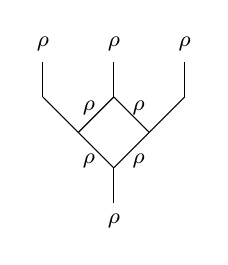
\begin{tikzpicture}[scale=0.45,baseline={(current bounding box.center)}]
					\draw (0,0) -- (0,1);
					\draw (0,1) -- (-1,2);
					\draw (0,1) -- (1,2);
					\draw (-1,2) -- (-2,3);
					\draw (-1,2) -- (0,3);
					\draw (1,2) -- (0,3);
					\draw (-2,3) -- (-2,4);
					\draw (0,3) -- (0,4);
					\draw (1,2) -- (2,3);
					\draw (2,3) -- (2,4);
					\node (1) at (0,-0.5) {\footnotesize $\rho$};
					\node (2) at (-2,4.5) {\footnotesize $\rho$};
					\node (3) at (0,4.5) {\footnotesize $\rho$};
					\node (4) at (-0.7,1.2) {\footnotesize $\rho$};
					\node (5) at (0.7,1.2) {\footnotesize $\rho$};
					\node (6) at (-0.7,2.7) {\footnotesize $\rho$};
					\node (7) at (0.7,2.7) {\footnotesize $\rho$};
					\node (8) at (2,4.5) {\footnotesize $\rho$};
				\end{tikzpicture}
			\end{equation}
		as an element in $\Hom(\rho,\rho\otimes\rho\otimes\rho)$ in the regular category $\Hd$ and applying $F$-moves to simplify it on the one hand, and comparing this to the corresponding relation \cref{eq:squarelincom} within the trivalent category (note that in the trivalent category, we can rotate strings and vertices without changing the value of a diagram). In the first case, we obtain the relation 
			\begin{equation}
				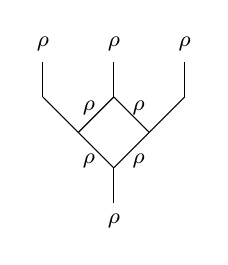
\begin{tikzpicture}[scale=.45,baseline=(current bounding box.center)]
					\draw (0,0) -- (0,1);
					\draw (0,1) -- (-1,2);
					\draw (0,1) -- (1,2);
					\draw (-1,2) -- (-2,3);
					\draw (-1,2) -- (0,3);
					\draw (1,2) -- (0,3);
					\draw (-2,3) -- (-2,4);
					\draw (0,3) -- (0,4);
					\draw (1,2) -- (2,3);
					\draw (2,3) -- (2,4);
					\node (1) at (0,-0.5) {\footnotesize $\rho$};
					\node (2) at (-2,4.5) {\footnotesize $\rho$};
					\node (3) at (0,4.5) {\footnotesize $\rho$};
					\node (4) at (-0.7,1.2) {\footnotesize $\rho$};
					\node (5) at (0.7,1.2) {\footnotesize $\rho$};
					\node (6) at (-0.7,2.7) {\footnotesize $\rho$};
					\node (7) at (0.7,2.7) {\footnotesize $\rho$};
					\node (8) at (2,4.5) {\footnotesize $\rho$};
				\end{tikzpicture}
				=\sum_{x} \big(F_\rho^{\rho\rho\rho}\big)^\dagger_{x \rho}\ \big(F_{x}^{\rho\rho\rho}\big)_{\rho\rho}\ \sqrt{d_\rho}\ 
				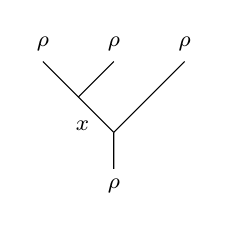
\begin{tikzpicture}[scale=.45,baseline=(current bounding box.center)]
					\node (u) at (6.5,-0.5) {\footnotesize $\rho$};
					\node (a) at (4.5,3.5) {\footnotesize $\rho$};
					\node (b) at (6.5,3.5) {\footnotesize $\rho$};
					\node (c) at (8.5,3.5) {\footnotesize $\rho$};
					\draw (u) -- (6.5,1);
					\draw (6.5,1) -- (8.5,3);
					\draw (5.5,2) -- (6.5,3);
					\draw (5.5,2) -- (4.5,3);
					\draw (6.5,1) -- (5.5,2) node[pos=0.2,left] {\footnotesize $x\ $};
				\end{tikzpicture}.
			\end{equation}
		Rewriting \cref{eq:squarelincom} as an equation in $\Hom(\rho,\rho\otimes\rho\otimes\rho)$ and bringing it into the same form as the equation above yields
			\begin{align}
				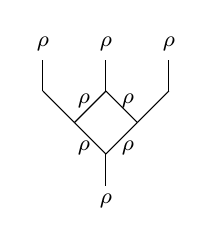
\begin{tikzpicture}[scale=.4,baseline=(current bounding box.center)]
					\draw (0,0) -- (0,1);
					\draw (0,1) -- (-1,2);
					\draw (0,1) -- (1,2);
					\draw (-1,2) -- (-2,3);
					\draw (-1,2) -- (0,3);
					\draw (1,2) -- (0,3);
					\draw (-2,3) -- (-2,4);
					\draw (0,3) -- (0,4);
					\draw (1,2) -- (2,3);
					\draw (2,3) -- (2,4);
					\node (1) at (0,-0.5) {\footnotesize $\rho$};
					\node (2) at (-2,4.5) {\footnotesize $\rho$};
					\node (3) at (0,4.5) {\footnotesize $\rho$};
					\node (4) at (-0.7,1.2) {\footnotesize $\rho$};
					\node (5) at (0.7,1.2) {\footnotesize $\rho$};
					\node (6) at (-0.7,2.7) {\footnotesize $\rho$};
					\node (7) at (0.7,2.7) {\footnotesize $\rho$};
					\node (8) at (2,4.5) {\footnotesize $\rho$};
				\end{tikzpicture}
				&=\alpha\ \left(
				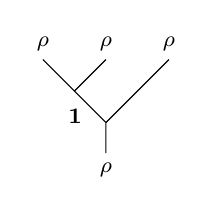
\begin{tikzpicture}[scale=.4,baseline=(current bounding box.center)]
					\node (u) at (6.5,-0.5) {\footnotesize $\rho$};
					\node (a) at (4.5,3.5) {\footnotesize $\rho$};
					\node (b) at (6.5,3.5) {\footnotesize $\rho$};
					\node (c) at (8.5,3.5) {\footnotesize $\rho$};
					\draw (u) -- (6.5,1);
					\draw (6.5,1) -- (8.5,3);
					\draw (5.5,2) -- (6.5,3);
					\draw (5.5,2) -- (4.5,3);
					\draw (6.5,1) -- (5.5,2) node[pos=0.2,left] {\footnotesize $\mathbf{1}\ $};
				\end{tikzpicture}
				+
				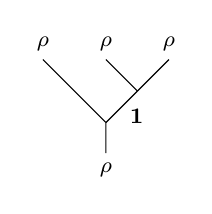
\begin{tikzpicture}[scale=.4,baseline=(current bounding box.center)]
					\node (u) at (6.5,-0.5) {\footnotesize $\rho$};
					\node (a) at (4.5,3.5) {\footnotesize $\rho$};
					\node (b) at (6.5,3.5) {\footnotesize $\rho$};
					\node (c) at (8.5,3.5) {\footnotesize $\rho$};
					\draw (u) -- (6.5,1);
					\draw (6.5,1) -- (7.5,2) node[pos=0.2,right] {\footnotesize $\ \mathbf{1}$};
					\draw (7.5,2) -- (6.5,3);
					\draw (7.5,2) -- (8.5,3);
					\draw (6.5,1) -- (4.5,3);
				\end{tikzpicture}
				\right) +\beta\ \left(
				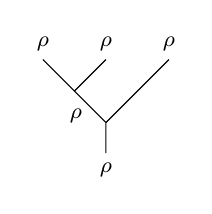
\begin{tikzpicture}[scale=.4,baseline=(current bounding box.center)]
					\node (u) at (6.5,-0.5) {\footnotesize $\rho$};
					\node (a) at (4.5,3.5) {\footnotesize $\rho$};
					\node (b) at (6.5,3.5) {\footnotesize $\rho$};
					\node (c) at (8.5,3.5) {\footnotesize $\rho$};
					\draw (u) -- (6.5,1);
					\draw (6.5,1) -- (8.5,3);
					\draw (5.5,2) -- (6.5,3);
					\draw (5.5,2) -- (4.5,3);
					\draw (6.5,1) -- (5.5,2) node[pos=0.2,left] {\footnotesize $\rho\ $};
				\end{tikzpicture}
				+
				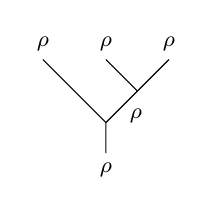
\begin{tikzpicture}[scale=.4,baseline=(current bounding box.center)]
					\node (u) at (6.5,-0.5) {\footnotesize $\rho$};
					\node (a) at (4.5,3.5) {\footnotesize $\rho$};
					\node (b) at (6.5,3.5) {\footnotesize $\rho$};
					\node (c) at (8.5,3.5) {\footnotesize $\rho$};
					\draw (u) -- (6.5,1);
					\draw (6.5,1) -- (7.5,2) node[pos=0.2,right] {\footnotesize $\ \rho$};
					\draw (7.5,2) -- (6.5,3);
					\draw (7.5,2) -- (8.5,3);
					\draw (6.5,1) -- (4.5,3);
				\end{tikzpicture}
				\right)\\
			&=\alpha\ \left(
				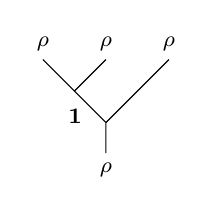
\begin{tikzpicture}[scale=.4,baseline=(current bounding box.center)]
					\node (u) at (6.5,-0.5) {\footnotesize $\rho$};
					\node (a) at (4.5,3.5) {\footnotesize $\rho$};
					\node (b) at (6.5,3.5) {\footnotesize $\rho$};
					\node (c) at (8.5,3.5) {\footnotesize $\rho$};
					\draw (u) -- (6.5,1);
					\draw (6.5,1) -- (8.5,3);
					\draw (5.5,2) -- (6.5,3);
					\draw (5.5,2) -- (4.5,3);
					\draw (6.5,1) -- (5.5,2) node[pos=0.2,left] {\footnotesize $\mathbf{1}\ $};
				\end{tikzpicture}
				+\sum_x \left(F_\rho^{\rho\rho\rho}\right)^\dagger_{x\mathbf{1}}\ 
				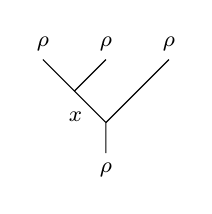
\begin{tikzpicture}[scale=.4,baseline=(current bounding box.center)]
					\node (u) at (6.5,-0.5) {\footnotesize $\rho$};
					\node (a) at (4.5,3.5) {\footnotesize $\rho$};
					\node (b) at (6.5,3.5) {\footnotesize $\rho$};
					\node (c) at (8.5,3.5) {\footnotesize $\rho$};
					\draw (u) -- (6.5,1);
					\draw (6.5,1) -- (8.5,3);
					\draw (5.5,2) -- (6.5,3);
					\draw (5.5,2) -- (4.5,3);
					\draw (6.5,1) -- (5.5,2) node[pos=0.2,left] {\footnotesize $x\ $};
				\end{tikzpicture}
				\right)\\
				&\hspace{40pt}+\beta\ \left(
				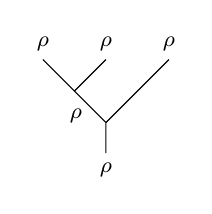
\begin{tikzpicture}[scale=.4,baseline=(current bounding box.center)]
					\node (u) at (6.5,-0.5) {\footnotesize $\rho$};
					\node (a) at (4.5,3.5) {\footnotesize $\rho$};
					\node (b) at (6.5,3.5) {\footnotesize $\rho$};
					\node (c) at (8.5,3.5) {\footnotesize $\rho$};
					\draw (u) -- (6.5,1);
					\draw (6.5,1) -- (8.5,3);
					\draw (5.5,2) -- (6.5,3);
					\draw (5.5,2) -- (4.5,3);
					\draw (6.5,1) -- (5.5,2) node[pos=0.2,left] {\footnotesize $\rho\ $};
				\end{tikzpicture}
				+\sum_x \left(F_\rho^{\rho\rho\rho}\right)^\dagger_{x\rho}\ 
				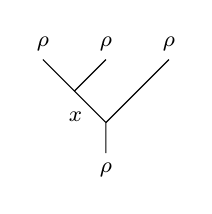
\begin{tikzpicture}[scale=.4,baseline=(current bounding box.center)]
					\node (u) at (6.5,-0.5) {\footnotesize $\rho$};
					\node (a) at (4.5,3.5) {\footnotesize $\rho$};
					\node (b) at (6.5,3.5) {\footnotesize $\rho$};
					\node (c) at (8.5,3.5) {\footnotesize $\rho$};
					\draw (u) -- (6.5,1);
					\draw (6.5,1) -- (8.5,3);
					\draw (5.5,2) -- (6.5,3);
					\draw (5.5,2) -- (4.5,3);
					\draw (6.5,1) -- (5.5,2) node[pos=0.2,left] {\footnotesize $x\ $};
			\end{tikzpicture}
			\right).
			\end{align}
		Comparing the different linear combinations of basis vectors for the diagram in question for $x={}_\alpha\rho$ and $x=\alphastarrho$ yields the statement of the proof.
	\end{proof}

	It is possible to exploit various other relations within the trivalent category to gain information about the $F$-symbols. A detailed list of these relations can be found in \cite{Osborne2019}. 
	
	The seed data generated by the methods described above provides enough information such that the set of equations becomes simple enough to be solvable with standard techniques. The $F$-symbols of the $\Hi_3$ category have also independently been obtained by Matthew Titsworth \cite{PrivateTitsworth}.


\section{Algebra objects in $\Hd$}

The $F$-symbols of a category can be exploited to find algebra objects and modules of the category. In this section, we describe how this procedure works by calculating an explicit example. As depicted in \cref{fig:MoritaH}, $\mathcal{H}_1$ can be constructed as the category $\mathsf{Bimod}_{\Hd}(A,A)$ with $A=\mathbf{1}+\rho+{}_\alpha\rho$. First, we show that $\mathbf{1}+\rho+{}_\alpha\rho$ is an algebra object in $\Hd$ by constructing the corresponding multiplication morphism.

The multiplication morphism $m:A\otimes A\to A$ is an element of the morphism space $\Hom(A\otimes A,A)$. To find out the dimension of this space, note that we can write $A=\mathbf{1}+\rho+{}_\alpha\rho$ as
	\begin{equation}
		A=\bigoplus_{X\in\Obj(\Hd)}a_XX,
	\end{equation}
where $\Obj(\Hd)=\{\mathbf{1},\alpha,\alpha^*,\rho,{}_\alpha\rho,\alphastarrho\}$ and $a_X=0$ for $X\in\{\alpha,\alpha^*,\alphastarrho\}$ and $a_X=1$ for $X\in\{\mathbf{1},\rho,{}_\alpha\rho\}$. Hence, the morphism space $\Hom(A\otimes A,A)$ can be written as a combination of morphism spaces only including simple objects:
	\begin{equation}
		\Hom(A\otimes A,A)=\bigoplus_{X,Y,Z\in\Obj(\Hd)}a_Xa_Ya_Z\Hom(X\otimes Y,Z).
	\end{equation}
To obtain the dimension of this space, we simply calculate
	\begin{equation}
		\dim(\Hom(A\otimes A,A))=\sum_{X,Y,Z\in\Obj(\Hd)} a_Xa_Ya_Z\dim(\Hom(X\otimes Y,Z))=15.
	\end{equation}
Therefore, an element $m\in\Hom(A\otimes A,A)$ is a linear combination of the $15$ basis diagrams of this space:
	\begin{align}
		m &= c_{\mathbf{1}\mathbf{1}}^\mathbf{1}\vertex{\mathbf{1}}{\mathbf{1}}{\mathbf{1}} + c_{\mathbf{1}\rho}^{\rho}\vertex{\mathbf{1}}{\rho}{\rho} + c_{\mathbf{1}{}_\alpha\rho}^{{}_\alpha\rho}\vertex{\mathbf{1}}{{}_\alpha\rho}{{}_\alpha\rho} + c_{\rho\mathbf{1}}^{\rho}\vertex{\rho}{\mathbf{1}}{\rho}+	c_{\rho\rho}^{\mathbf{1}}\vertex{\rho}{\rho}{\mathbf{1}}\\ \label{eq:mdecomp} &\hspace{10pt} + c_{\rho\rho}^{\rho}\vertex{\rho}{\rho}{\rho} + c_{\rho\rho}^{{}_\alpha\rho}\vertex{\rho}{\rho}{{}_\alpha\rho} + c_{\rho{}_\alpha\rho}^{\rho}\vertex{\rho}{{}_\alpha\rho}{\rho}+c_{\rho{}_\alpha\rho}^{{}_\alpha\rho}\vertex{\rho}{{}_\alpha\rho}{{}_\alpha\rho}  + c_{{}_\alpha\rho \mathbf{1}}^{ {}_\alpha\rho}\vertex{{}_\alpha\rho}{\mathbf{1}}{{}_\alpha\rho}\\&\hspace{10pt}+ c_{{}_\alpha\rho\rho}^{\rho}\vertex{{}_\alpha\rho}{\rho}{\rho} + c_{{}_\alpha\rho\rho}^{ {}_\alpha\rho}\vertex{{}_\alpha\rho}{\rho}{{}_\alpha\rho}+  
		c_{{}_\alpha\rho  {}_\alpha\rho}^{ \mathbf{1}}\vertex{{}_\alpha\rho}{{}_\alpha\rho}{\mathbf{1}} + c_{{}_\alpha\rho  {}_\alpha\rho}^{\rho}\vertex{{}_\alpha\rho}{{}_\alpha\rho}{\rho} + c_{{}_\alpha\rho  {}_\alpha\rho}^{ {}_\alpha\rho}\vertex{{}_\alpha\rho}{{}_\alpha\rho}{{}_\alpha\rho}.
	\end{align}
In order to find the multiplication morphism $m$ for the algebra object, all $15$ coefficients have to be determined. To solve this problem, we can make use of the different conditions that this morphism has to fulfil (see \cref{def:algebraobject}). Condition \cref{eq:AO2} already fixes five of the coefficients:
	\begin{equation}
		c_{\mathbf{1}\mathbf{1}}^\mathbf{1}=c_{\mathbf{1}\rho}^{\rho}=c_{\mathbf{1}{}_\alpha\rho}^{{}_\alpha\rho}=c_{\rho\mathbf{1}}^\rho=c_{{}_\alpha\rho\mathbf{1}}^{{}_\alpha\rho}=1.
	\end{equation}
This leaves us with $10$ unknowns. Additional equations that help us to determine these coefficients come from condition \cref{eq:AO1} of the definition: Inserting the decomposition \cref{eq:mdecomp} into \cref{eq:mcondpic} yields a linear combination of $81$ terms for the left hand side of the equation:
	\begin{align}
		\begin{tikzpicture}[scale=0.75,baseline=(current bounding box.center)]
			\draw (0,0) to (90:1);
			\draw (0,0) to (230:1);
			\draw (0,0) to (310:1);	
			\draw[fill=LinkColor2!50!white] (0,0) circle(0.35cm);	
			\node (c) at (0,0) {\small $m$};
			\node at (90:1.25) {\small $A$};	
			\node at (230:1.25) {\small $A$};
			\node at (310:1.25) {\small $A$};	
			\begin{scope}[yshift=2.2cm, xshift=0.9cm]
			\draw (0,0) to (90:1);
			\draw (0,0) to (230:1);
			\draw (0,0) to (295:3.225);	
			\draw[fill=LinkColor2!50!white] (0,0) circle(0.35cm);	
			\node (c) at (0,0) {\small $m$};
			\node at (90:1.25) {\small $A$};	
			\node at (295:3.475) {\small $A$};	
			\end{scope}
		\end{tikzpicture}&={c_{\mathbf{1}\mathbf{1}}^\mathbf{1}}^2\fuselefttree{\mathbf{1}}{\mathbf{1}}{\mathbf{1}}{\mathbf{1}}{\mathbf{1}}+c_{\mathbf{1}\mathbf{1}}^\mathbf{1}c_{\mathbf{1}\rho}^\rho\fuselefttree{\mathbf{1}}{\mathbf{1}}{\mathbf{1}}{\rho}{\rho}+c_{\mathbf{1}\mathbf{1}}^\mathbf{1}c_{\mathbf{1}{}_\alpha\rho}^{{}_\alpha\rho}\fuselefttree{\mathbf{1}}{\mathbf{1}}{\mathbf{1}}{{}_\alpha\rho}{{}_\alpha\rho}\\
		&\hspace{10pt}+c_{\mathbf{1}\rho}^\rho c_{\rho\rho}^\mathbf{1}\fuselefttree{\mathbf{1}}{\rho}{\rho}{\rho}{\mathbf{1}} +c_{\mathbf{1}\rho}^\rho c_{\rho \mathbf{1}}^\rho\fuselefttree{\mathbf{1}}{\rho}{\rho}{\mathbf{1}}{\rho}+c_{\mathbf{1}\rho}^\rho c_{\rho\rho}^\rho\fuselefttree{\mathbf{1}}{\rho}{\rho}{\rho}{\rho}+\dots
	\end{align}
and the same number of terms for the right hand side. We can now work out a general form for the equations that can be deduced from this condition: Note that the general form of the terms on the left hand side of the equation is
	\begin{equation}
		c_{xy}^\alpha c_{\alpha z}^w\fuselefttree{x}{y}{\alpha}{z}{w},		
	\end{equation}
where we call this kind of diagram a \emph{left fusion tree}. If the morphism space $\Hom(x\otimes y\otimes z,w)$ is one-dimensional, making a basis transformation by applying the corresponding $F$-move\footnote{Note that these fusion trees are mirrored horizontally compared to the diagrams that appear in the construction of $F$-symbols. Hence, in general, we have to use the complex conjugate of the entries of the $F$-matrix here (see \cref{sec:alganyons}). However, since the $F$-symbols are real for the $\Hi$ category (see \cref{app:Fsymbols}), we can use the standard $F$-symbols here.} yields
	\begin{equation}
	\label{eq:mmorphcond}
		c_{xy}^\alpha c_{\alpha z}^w\fuselefttree{x}{y}{\alpha}{z}{w}=c_{xy}^\alpha c_{\alpha z}^w\left(F_w^{xyz}\right)_{\beta\alpha}\fuserighttree{x}{y}{\beta}{z}{w}
	\end{equation}
On the right hand side of the equation, there will be a term of the form
	\begin{equation}
		c_{x\beta}^w c_{y z}^\beta\fuserighttree{x}{y}{\beta}{z}{w}
	\end{equation}
(a \emph{right fusion tree}) since there is one term for each basis diagram of the morphism space. Comparing the coefficients of the two terms yields the condition
	\begin{equation}
	\label{eq:condm}
		c_{xy}^\alpha c_{\alpha z}^w\left(F_w^{xyz}\right)_{\beta\alpha}=c_{x\beta}^w c_{y z}^\beta.
	\end{equation}
This procedure can easily be generalized to higher-dimensional morphism spaces. In this case, there will be a sum over the label $\beta$ on the right hand side of \cref{eq:mmorphcond}, i.e., a sum over right fusion trees. This implies that every right fusion tree can come from more than one of the left fusion trees. Hence, we have to take sum over all left fusion trees which can give rise to a right fusion tree with label $\beta$ and the general form of condition \cref{eq:condm} is
	\begin{equation}
 		\sum_\alpha c_{xy}^\alpha c_{\alpha z}^w\left(F_w^{xyz}\right)_{\beta\alpha}=c_{x\beta}^w c_{y z}^\beta.
	\end{equation}
Solving this set of equations gives the following solution:
	\begin{align}
		c_{\rho {}_\alpha\rho}^{\rho}&=c_{\alpharho\rho}^\rho\\
		c_{{}_\alpha\rho \rho}^{{}_\alpha\rho}&=c_{\rho\alpharho}^\alpharho\\
		c_{\rho\rho}^\mathbf{1}&=\sqrt{\frac{1}{2} \left(3-\sqrt{2 \sqrt{13}-5}\right)}\ {c_{\rho{}_\alpha\rho}^{{}_\alpha\rho}}^2\\
		c_{{}_\alpha\rho {}_\alpha\rho}^\mathbf{1}&=-\sqrt{\frac{1}{2} \left(3+\sqrt{2 \sqrt{13}-5}\right)}\ p_1\  {c_{\alpharho\rho}^\rho}^2\\
		c_{{}_\alpha\rho {}_\alpha\rho}^\rho&=-\frac{1}{4}\left(1+\sqrt{13}+\sqrt{2 \left(\sqrt{13}-1\right)}\right)\ p_1\ \frac{{c_{\alpharho \rho}^{\rho}}^2}{c_{\rho\alpharho}^\alpharho}\\
		c_{\rho \rho}^{{}_\alpha\rho}&=-\frac{1}{4}\left(1+\sqrt{13}+\sqrt{2 \left(\sqrt{13}-1\right)}\right)\ p_1\ \frac{{c_{\rho \alpharho}^{\alpharho}}^2}{c_{\alpharho\rho}^\rho}\\
		c_{\rho \rho}^\rho&=\frac{1}{4} \left(3-\sqrt{13}-\sqrt{2 \left(\sqrt{13}-1\right)}\right)\ c_{\rho {}_\alpha\rho}^\alpharho\\
		c_{{}_\alpha\rho {}_\alpha\rho}^{{}_\alpha\rho}&=\frac{1}{4} \left(3-\sqrt{13}+\sqrt{2 \left(\sqrt{13}-1\right)}\right)c_{\rho {}_\alpha\rho}^\rho,
	\end{align}
where $p_1\in\{-1,+1\}$ is a parameter coming from the solution of the $F$-symbols in \cref{app:Fsymbols}. Note that two of the coefficients, $c_{\rho\alpharho}^\alpharho$ and $c_{\alpharho\rho}^\rho$ are not determined by the conditions.


\section{Module categories over $\Hd$}

In the previous chapter, we have shown how to construct module categories from algebra objects. Starting from the algebra object $A=\mathbf{1}+\rho+\alpharho$ we now show how to practically determine the category of left modules over $A$ in $\Hd$, following the same techniques we described in \cref{ex:FibMod}. We begin by determining the simple module objects via calculating the matrix $T$. Remember that a row of $T$ is given by the outcome of the fusion product $A\otimes X_i$ for $X_i\in\{\mathbf{1},\alpha,\alpha^*,\rho,\alpharho,\alphastarrho\}$, where the coefficients in the decomposition into simple objects are the entries in the row corresponding to the object $X_i$. The resulting matrix is
	\begin{equation}
		T=\begin{blockarray}{ccccccc}
		& 1 & \alpha & \alpha^* & \rho & {}_\alpha\rho & \alphastarrho\\
		\begin{block}{c (cccccc)}
		1 & 1 & 0 & 0 & 1 & 1 & 0 \topstrut \\
		\alpha & 0 & 1 & 0 & 1 & 0 & 1\\
		\alpha^* & 0 & 0 & 1 & 0 & 1 & 1\\
		\rho & 1 & 1 & 0 & 3 & 2 & 2\\
		{}_\alpha\rho & 1 & 0 & 1 & 2 & 3 & 2\\
		\alphastarrho & 0 & 1 & 1 & 2 & 2 & 3\botstrut \\
		\end{block}
		\end{blockarray}\ .
	\end{equation} 
Recall that $T$ can be rewritten as $T=VV^T$. Hence, $V$ is given by 
	\begin{equation}
		V=\begin{pmatrix}
		1 & 0 & 0 & 0\\
		0 & 1 & 0 & 0\\
		0 & 0 & 1 & 0\\
		1 & 1 & 0 & 1\\
		1 & 0 & 1 & 1\\
		0 & 1 & 1 & 1
		\end{pmatrix}.
	\end{equation}
We can directly conclude that there are four simple module objects in the category $\mathrm{Mod}_{\mathcal{H}_3}(A)$, which are
	\begin{align}
		M_1&=1+\rho+{}_\alpha\rho\\
		M_2&=\alpha+\rho+\alphastarrho\\
		M_3&=\alpha^*+{}_\alpha\rho+\alphastarrho\\
		M_4&=\rho+{}_\alpha\rho+\alphastarrho.
	\end{align}
The corresponding morphisms $l_{M_i}$ can be determined from the conditions given in \cref{def:leftmod} analogously to the calculation of the multiplication morphism $m$ of the algebra object.
	